%%%%%%%%%%%%%%%%%%%%%%%%%%%%%%%%%%%%%%%%%%%%%%%%%%%%%%%%%%%%%%%
%PANDOC SPECIFIC SHIT, TAKEN FROM ANOTHER TEMPLATE...

\documentclass[11pt,]{article}

%Deal with margins and other geometry stuff
\usepackage[margin = 1in]{geometry}
\usepackage{longtable}
\usepackage{booktabs}

% Need to include this for refs with Pandoc

%Some of this is math package stuff, but honestly i don't really get
%what most of it is doing
\usepackage{amssymb,amsmath}
\usepackage{ifxetex,ifluatex}
\usepackage{fixltx2e} % provides \textsubscript

%Numbered section spacing
\setcounter{secnumdepth}{0}

\usepackage{setspace}
\setstretch{1}

%For LIST (enumerate) spacing
\providecommand{\tightlist}{%
  \setlength{\itemsep}{0pt}\setlength{\parskip}{0pt}}

%%%%%%%%%%%%%%%%%%%%%%%%%%%%%%%%%%%%%%%%%%%%%%%%%%%%%%%%%%%%%%%%%%%
%% LUCY'S DOCUMENT PREAMBLE AND PACKAGES

\usepackage{pdflscape}
\usepackage{xcolor}

\usepackage{tcolorbox}
\newtcolorbox{blackbox}{
  colback=white,
  colframe=black,
  coltext=black,
  boxsep=5pt,
  arc=4pt}

%\usepackage[round]{natbib}
\usepackage[sectionbib, natbibapa]{apacite} 
\usepackage[hyphens]{url}

%Set paragraph indent and between paragraph spacing
\usepackage{parskip}
\setlength\parindent{0pt}
\setlength{\parskip}{0pt}

%Need all these for graphics and tables
\usepackage{subfig}
\usepackage{graphicx}
\usepackage{blindtext}
\usepackage{array}
\usepackage{float}

%Deal with titles and make them less stupid and ugly
\usepackage{titlesec}
\titleformat{\section}[block]{\bfseries\sc\filcenter}{}{1em}{}
%\titleformat{\section}[block]{\Large\bfseries\filcenter}{}{1em}{}
\titleformat{\subsection}[hang]{\bfseries}{}{1em}{}
\setcounter{secnumdepth}{0}

\usepackage[hyphens]{url}

%Bunch of hyperlink shit
\usepackage{hyperref}
\hypersetup{
    colorlinks=true,
    linkcolor=blue,
    filecolor=magenta,      
    urlcolor=cyan,
    citecolor = black
}


%Header and footer junk
\usepackage{fancyhdr}
\pagestyle{fancy}
\fancyhead[L,C]{}
\fancyhead[R]{\small{\textsc{L E Delaney} \hspace{3mm} \textit{Chapters
3 \& 4 Homework}}}
\fancyfoot[L]{\tiny{\textit{Version date: \today}}}
    \fancyfoot[R]{\thepage}
\fancyfoot[C]{}


%%%%%%%%%%%%%%%%%%%%%%%%%%%%%%%%%%%%%%%%%%%%%%%%%%%%%%%%%%%%%%%%%%%%%%%
%% START OF THE DOCUMENT BODY
\begin{document}

%%%%%% TITLE 
\begin{center}
\Large{\textsc{Chapters 3 \& 4 Homework}}\\ \small{\textit{Ch.3: 12, 13,
15, 20, 25a, 28, 30; Ch.4: 12-15, 18, 22, 23, 45}}\\
\vspace*{\baselineskip}
\end{center}

%%%%%%%%%%%%%% DOCUMENT BODY
\begin{blackbox}

\begin{enumerate}
\def\labelenumi{\arabic{enumi}.}
\setcounter{enumi}{11}
\tightlist
\item
  Assume independent assortment and start with a plant that is dihybrid
  \emph{A/a ; B/b}.

  \begin{enumerate} 
   \item[a.]{ What phenotypic ratio is produced from selfing it? } 
   \item[b.]{ What genotypic ratio is produced from selfing it? } 
   \item[c.]{ What phenotypic ratio is produced from testcrossing it? } 
   \item[d.]{ What genotypic ratio is produced from testcrossing it? } 
   \end{enumerate}
\end{enumerate}

\vspace{17cm}

\end{blackbox}

\begin{blackbox}

\begin{enumerate}
\def\labelenumi{\arabic{enumi}.}
\setcounter{enumi}{12}
\tightlist
\item
  Normal mitosis takes place in a diploid cell of genotype \emph{A/a ;
  B/b}. Which of the following genotypes might represent possible
  daughter cells?
\end{enumerate}

\hfill\break

\begin{enumerate}
\def\labelenumi{\alph{enumi}.}
\item
  \emph{A;B}
\item
  \emph{a;b}
\item
  \emph{A;b}
\item
  \emph{a;B}
\item
  \emph{A/A ; B/B}
\item
  \emph{A/a ; B/b}
\item
  \emph{a/a ; b/b}
\end{enumerate}

\vspace{15cm}

\end{blackbox}

\begin{blackbox}

\begin{enumerate}
\def\labelenumi{\arabic{enumi}.}
\setcounter{enumi}{14}
\tightlist
\item
  It has been shown that, when a thin beam of light is aimed at a
  nucleus, the amount of light absorbed is proportional to the cell's
  DNA content. Using this method, the DNA in the nuclei of several
  different types of cells in a corn plant were compared. The following
  numbers represent the relative amounts of DNA in these different types
  of cells:
\end{enumerate}

\vspace{10mm}

\begin{center}

0.7, 1.4, 2.1, 2.8, and 4.2

\vspace{10mm}
\end{center}

Which cells could have been used for these measurements? (Note: In
plants, the endosperm part of the seed is often triploid, 3n.)

\vspace{14cm}

\end{blackbox}

\begin{blackbox}

\begin{enumerate}
\def\labelenumi{\arabic{enumi}.}
\setcounter{enumi}{19}
\tightlist
\item
  In mice, dwarfism is caused by an X-linked recessive allele, and pink
  coat is caused by an autosomal dominant allele (coats are normally
  brownish). If a dwarf female from a pure line is crossed with a pink
  male from a pure line, what will be the phenotypic ratios in the F1
  and F2 in each sex? (Invent and define your own gene symbols.)
\end{enumerate}

\vspace{19cm}

\end{blackbox}

\begin{blackbox}

\begin{enumerate}
\def\labelenumi{\arabic{enumi}.}
\setcounter{enumi}{24}
\tightlist
\item
  Look at the Punnett square in Figure 3-4. (Only part a is assigned.)
\end{enumerate}

\begin{enumerate} 
 \item[a.]{ How many genotypes are there in the 16 squares of the grid? } 
 \item[b.]{ What is the genotypic ratio underlying the 9:3:3:1 phenotypic ratio? } 
 \item[c.]{ Can you devise a simple formula for the calculation of the number of progeny genotypes in dihybrid, trihybrid, and so forth crosses? Repeat for phenotypes. } 
 \item[d.]{ Mendel predicted that, within all but one of the phenotypic classes in the Punnett square, there should be several different genotypes. In particular, he performed many crosses to identify the underlying genotypes of the round, yellow phenotype. Show two different ways that could be used to identify the various genotypes underlying the round, yellow phenotype. (Remember, all the round, yellow peas look identical.) } 
 \end{enumerate}

\hfill\break

\begin{center}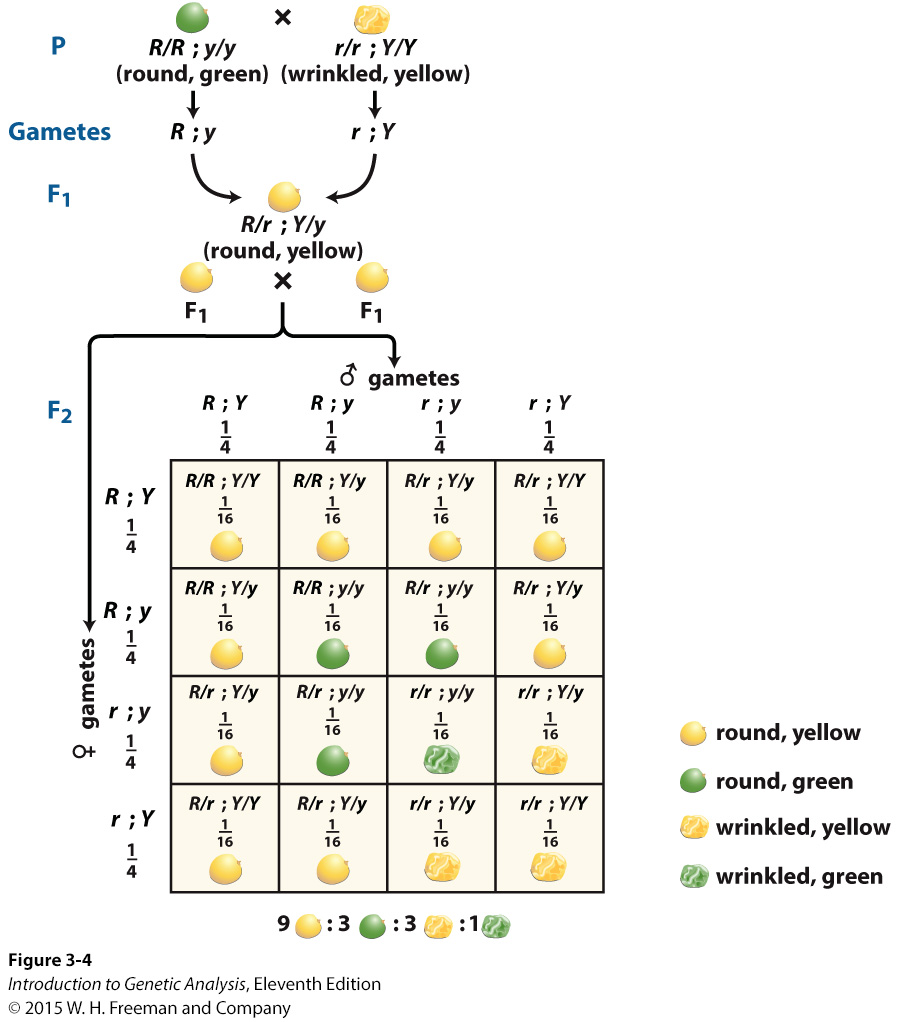
\includegraphics[width=0.45\linewidth,]{input/figure_03_04} \end{center}

\vspace{8cm}

\end{blackbox}

\begin{blackbox}

\begin{enumerate}
\def\labelenumi{\arabic{enumi}.}
\setcounter{enumi}{27}
\tightlist
\item
  In dogs, dark coat color is dominant over albino and short hair is
  dominant over long hair. Assume that these effects are caused by two
  independently assorting genes. Seven crosses were done as shown below,
  in which D and A stand for the dark and albino phenotypes,
  respectively, and S and L stand for the short-hair and long-hair
  phenotypes.
\end{enumerate}

\hfill\break

\begin{longtable}[]{@{}lllll@{}}
\toprule
Parental pheno. & D, S & D, L & A, S & A, L\tabularnewline
\midrule
\endhead
D, S x D, S & 88 & 31 & 29 & 12\tabularnewline
D, S x D, L & 19 & 18 & 0 & 0\tabularnewline
D, S x A, S & 21 & 0 & 20 & 0\tabularnewline
A, S x A, S & 0 & 0 & 29 & 9\tabularnewline
D, L x D, L & 0 & 31 & 0 & 11\tabularnewline
D, S x D, S & 45 & 16 & 0 & 0\tabularnewline
D, S x D, L & 31 & 30 & 10 & 10\tabularnewline
\bottomrule
\end{longtable}

\begin{center}\rule{0.5\linewidth}{0.5pt}\end{center}

\vspace{12cm}

\end{blackbox}

\begin{blackbox}

\begin{enumerate}
\def\labelenumi{\arabic{enumi}.}
\setcounter{enumi}{29}
\tightlist
\item
  A mutant allele in mice causes a bent tail. Six pairs of mice were
  crossed. Their phenotypes and those of their progeny are given in the
  following table. N is normal phenotype; B is bent phenotype. Deduce
  the mode of inheritance of this phenotype.
\end{enumerate}

\hfill\break

\begin{longtable}[]{@{}lllll@{}}
\toprule
& & PARENTS & & PROGENY\tabularnewline
\midrule
\endhead
Cross & Female & Male & Female & Male\tabularnewline
----- & --------- & ------- & ------- & -------\tabularnewline
1 & N & B & All B & All N\tabularnewline
2 & B & N & 1/2B 1/2N & 1/2B 1/2N\tabularnewline
3 & B & N & All B & All B\tabularnewline
4 & N & N & All N & All N\tabularnewline
5 & B & B & All B & All B\tabularnewline
6 & B & B & All B & 1/2B 1/2N\tabularnewline
\bottomrule
\end{longtable}

\begin{enumerate} 
 \item[a.]{ Is it recessive or dominant? } 
 \item[b.]{ Is it autosomal or sex-linked? } 
 \item[c.]{ What are the genotypes of all parents and progeny? } 
 \end{enumerate}

\begin{center}\rule{0.5\linewidth}{0.5pt}\end{center}

\vspace{12cm}

\end{blackbox}

\begin{blackbox}

\begin{enumerate}
\def\labelenumi{\arabic{enumi}.}
\setcounter{enumi}{11}
\tightlist
\item
  A plant of genotype
\end{enumerate}

\hfill\break

\begin{verbatim}
___A____B___
___a____b___
\end{verbatim}

\hfill\break

is testcrossed with

\begin{verbatim}
___a____b___
___a____b___
\end{verbatim}

\hfill\break

If the two loci are 10 m.u. apart, what proportion of progeny will be
\emph{A B / a b}?

\vspace{15cm}

\end{blackbox}

\begin{blackbox}

\begin{enumerate}
\def\labelenumi{\arabic{enumi}.}
\setcounter{enumi}{12}
\tightlist
\item
  The \emph{A} locus and the \emph{D} locus are so tightly linked that
  no recombination is ever observed between them. If \emph{A d / A d} is
  crossed with \emph{a D / a D} and the F1 is intercrossed, what
  phenotypes will be seen in the F2 and in what proportions?
\end{enumerate}

\vspace{19cm}

\end{blackbox}

\begin{blackbox}

\begin{enumerate}
\def\labelenumi{\arabic{enumi}.}
\setcounter{enumi}{13}
\tightlist
\item
  The \emph{R} and \emph{S} loci are 35 m.u. apart. If a plant of
  genotype
\end{enumerate}

\hfill\break

\begin{verbatim}
___R____S___
\end{verbatim}

\hfill\break

\begin{verbatim}
___r____s___
\end{verbatim}

\hfill\break

is selfed, what progeny phenotypes will be seen and in what proportions?

\vspace{15cm}

\end{blackbox}

\begin{blackbox}

\begin{enumerate}
\def\labelenumi{\arabic{enumi}.}
\setcounter{enumi}{14}
\tightlist
\item
  The cross \emph{E/E · F/F} x \emph{e/e · f/f} is made, and the F1 is
  then backcrossed with the recessive parent. The progeny genotypes are
  inferred from the phenotypes. The progeny genotypes, written as the
  gametic contributions of the heterozygous parent, are in the following
  proportions:
\end{enumerate}

\hfill\break

\emph{E·F} 2/6

\emph{E·f} 1/6

\emph{e·F} 1/6

\emph{e·f} 2/6

~

Explain these results.

\vspace{15cm}

\end{blackbox}

\begin{blackbox}

\begin{enumerate}
\def\labelenumi{\arabic{enumi}.}
\setcounter{enumi}{17}
\tightlist
\item
  If \emph{A/A · B/B} is crossed with \emph{a/a · b/b} and the F1 is
  testcrossed, what percentage of the testcross progeny will be
  \emph{a/a · B/b} if the two genes are \textbf{(a)} unlinked;
  \textbf{(b)} completely linked (no crossing over at all); \textbf{(c)}
  10 m.u. apart; \textbf{(d)} 24 m.u. apart?
\end{enumerate}

\vspace{19cm}

\end{blackbox}

\begin{blackbox}

\begin{enumerate}
\def\labelenumi{\arabic{enumi}.}
\setcounter{enumi}{21}
\tightlist
\item
  You have a Drosophila line that is homozygous for autosomal recessive
  alleles a, b, and c, linked in that order. You cross females of this
  line with males homozygous for the corresponding wild-type alleles.
  You then cross the F1 heterozygous males with their heterozygous
  sisters. You obtain the following F2 phenotypes (where letters denote
  recessive phenotypes and pluses denote wild-type phenotypes):
\end{enumerate}

\begin{center}

1364 + + + 

365 a b c

87 a b +

84 + + c

47 a + +

44 + b c

5 a + c

4 + b +

\end{center}

\begin{enumerate} 
 \item[a.]{ What is the map distance between a and b? Between b and c? (Remember, there is no crossing over in Drosophila males.) } 
 \item[b.]{ What is the coefficient of coincidence? } 
 \end{enumerate}

\vspace{12cm}

\end{blackbox}

\begin{blackbox}

\begin{enumerate}
\def\labelenumi{\arabic{enumi}.}
\setcounter{enumi}{22}
\tightlist
\item
  R. A. Emerson crossed two different pure-breeding lines of corn and
  obtained a phenotypically wild-type F1 that was heterozygous for three
  alleles that determine recessive phenotypes: \emph{an} determines
  anther; \emph{br}, brachytic; and \emph{f}, fine. He testcrossed the
  F1 with a tester that was homozygous recessive for the three genes and
  obtained these progeny phenotypes: 355 anther; 339 brachytic, fine; 88
  completely wild type; 55 anther, brachytic, fine; 21 fine; 17 anther,
  brachytic; 2 brachytic; 2 anther, fine.
\end{enumerate}

\begin{enumerate} 
 \item[a.]{ What were the genotypes of the parental lines? } 
 \item[b.]{ Draw a linkage map for the three genes (include map distances). } 
 \item[c.]{ Calculate the interference value. } 
 \end{enumerate}

\vspace{15cm}

\end{blackbox}

\begin{blackbox}

\begin{enumerate}
\def\labelenumi{\arabic{enumi}.}
\setcounter{enumi}{44}
\tightlist
\item
  A corn geneticist wants to obtain a corn plant that has the three
  dominant phenotypes: anthocyanin (A), long tassels (L), and dwarf
  plant (D). In her collection of pure lines, the only lines that bear
  these alleles are \emph{AA LL dd} and \emph{aa ll DD}. She also has
  the fully recessive line \emph{aa ll dd}. She decides to intercross
  the first two and testcross the resulting hybrid to obtain in the
  progeny 0 plant of the desired phenotype (which would have to be
  \emph{Aa Ll Dd} in this case). She knows that the three genes are
  linked in the order written and that the distance between the
  \emph{A/a} and the \emph{L/l} loci is 16 map units and that the
  distance between the \emph{L/l} and the \emph{D/d} loci is 24 map
  units.
\end{enumerate}

\vspace{17cm}

\end{blackbox}

\end{document}


